\chapter{工具实现}
\label{ch5}

\section{异构系统验证分析工具(Co-SMC)介绍}
在本文我们提出了一种面向异构系统的验证分析方法,该方法基于协同仿真和统计模型检测,实现对异构系统行为的验证、分析。为了对该方法提供支持,我们设计、开发了异构系统验证分析工具,该工具主要由协同仿真、统计模型检测器及统计分析器三部分组成。在协同仿真器模块中,用户可以输入要进行协同仿真的多个FMU模型,然后设置仿真步长和多个FMU模型之间的参数对应关系,最后,可以从4种协同仿真算法中选择适当的协同仿真算法,对系统模型进行协同仿真并产生协同仿真的迹。统计模型检测器模块以协同仿真器产生的迹为输入,然后设置需要验证的属性,最后选择适合的统计模型检测算法进行定量的验证分析。用户可以在统计分析器模块对协同仿真器产生的迹或是统计模型检测器产生的验证结果进行统计分析,并绘制出饼状图、折线图等可视化的图形,有利于对模型的各种行为进行更加直观的分析。接下来我们对Co-SMC工具的各个部分进行详细的描述。
\begin{figure}[htbp]
	\centering
	{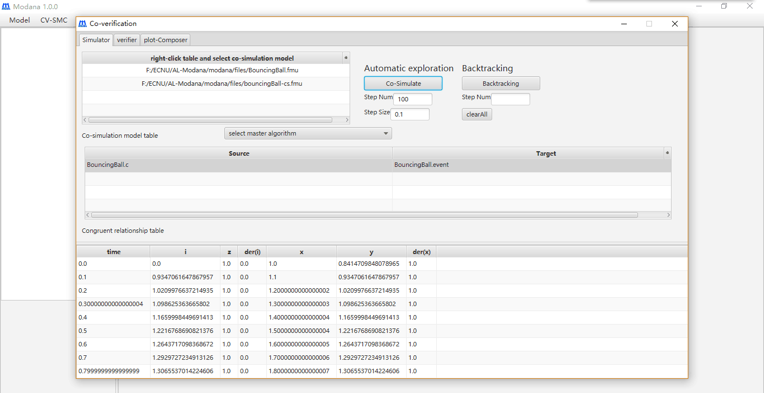
\includegraphics[width=4.0in]{fig/5/tool1.png}}
	%\vspace{0.10in}
	\caption{Co-SMC协同仿真器}\label{tool-1}
\end{figure}
\begin{figure}[htbp]
	\centering
	{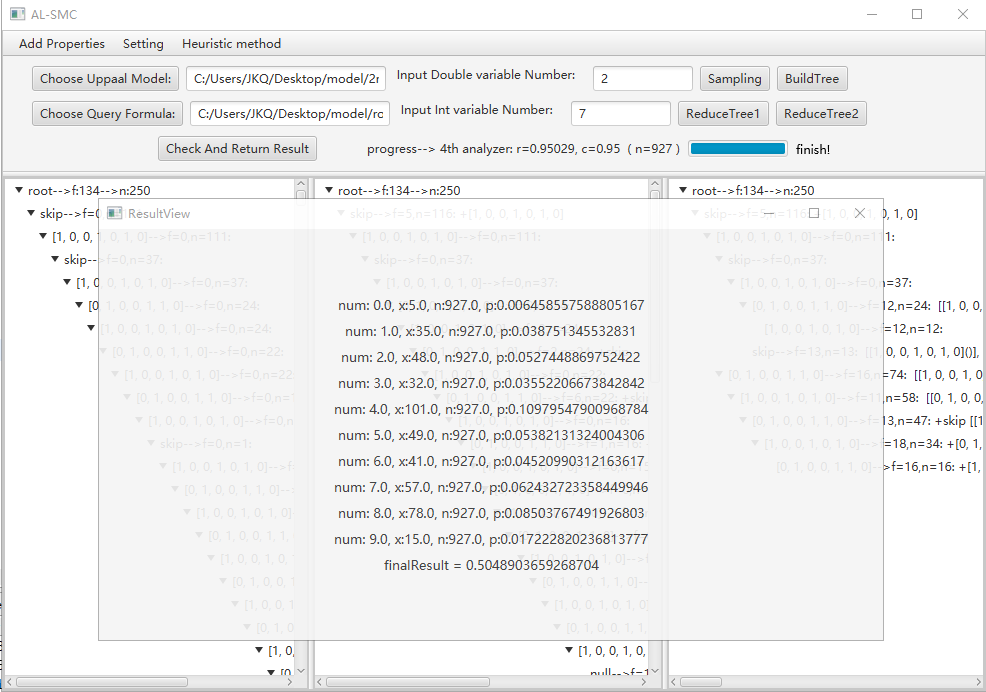
\includegraphics[width=4.0in]{fig/5/tool2.png}}
	%\vspace{0.10in}
	\caption{Co-SMC统计模型检测器}\label{tool-2}
\end{figure}
\begin{figure}[htbp]
	\centering
	{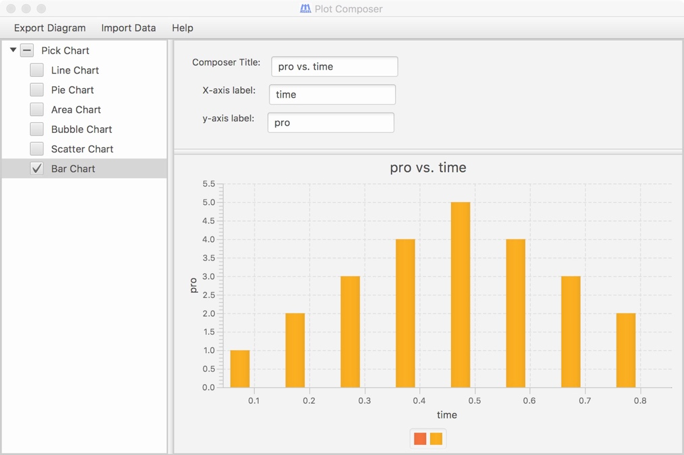
\includegraphics[width=4.0in]{fig/5/tool3.png}}
	%\vspace{0.10in}
	\caption{Co-SMC协同仿真器}\label{tool-3}
\end{figure}
图\ref{tool-1}是Co-SMC工具的协同仿真器,该工具主要包括
\section{Co-SMC程序实现}


\section{本章小结}
